\subsection{RQ1: Probability Variation}

\begin{figure} 
  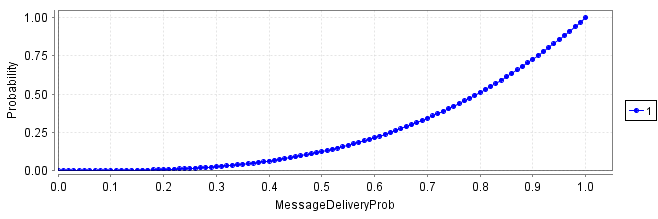
\includegraphics[width=\textwidth]{RQ1-small.png}
  \caption{Probability of Property Satisfied vs Message Success Probability}
  \label{RQ1-small}
\end{figure}

For this set of experiments the number of retries is set to 1. The probability of successful message delivery is varied and probability of property violation is observed. For small model it is possible to use PRISM's analytical solver to get exact probabilities. Since we used analytical solver for this model, no time bound is specified. The results are presented in Figure \ref{RQ1-small}. The figure clearly shows that the safety property holds more certainly when messages are more likely to be delivered. We expected the trend of rapid increase towards the end because multiple messages are required to achieve consistency in our model. If just one message was required we would have expected a straight line.

\begin{figure} 
  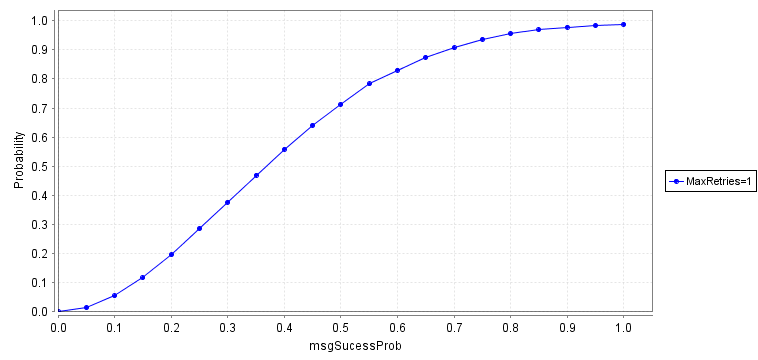
\includegraphics[width=\textwidth]{RQ1-large.png}
  \caption{Probability of Property Satisfied vs Message Success Probability}
  \label{RQ1-large}
\end{figure}

For the larger model we are computing the probability of catching a burglar given that the burglar in the house. For this experiment we are using simulation approach because solving this analytically is not feasible as discussed earlier. The simulations are bounded so we consider a simulated path length of 110 and a time bound of 100 for burglar to be identified and caught. The number of samples for each simulation is set to 25000. The results are shown in Figure \ref{RQ1-large}. The shape of the graph is different from the shape observed with the small model. This is because the small model has a simple series of messages that should pass in sequence to achieve consistency. Here the burglar can be detected by any of the 5 sensors. This introduces redundancy in the system and result in a probability of detection which is higher than the probability of successful delivery of a single message. We observe that the probability of system success surpasses the probability of successful message delivery at around 0.2. 